\documentclass[11pt,a4paper]{article}
\usepackage[T1]{fontenc}
\usepackage[utf8]{inputenc}
\usepackage[french]{babel}
\usepackage{lmodern}
\usepackage{geometry}
\usepackage{amsmath,amssymb}
\usepackage{booktabs}
\usepackage{graphicx}
\usepackage{hyperref}
\geometry{margin=2.4cm}

\title{Rapport round 4\\
\large Pont predictif minimal pour le WIP: $\beta_k$, point fixe de population, fragilite cachee et diagnostic spectral}
\author{Codex}
\date{9 avril 2026}

\begin{document}
\maketitle

\begin{abstract}
Le round 3 avait clarifie les observables et separe flux et stocks, mais il restait trop descriptif pour justifier le mot ``predictif''. Le round 4 ne ferme pas tout le champ moyen; il construit un pont predictif minimal sur quatre objets. Premierement, le taux tardif de creation de credit par entite vivante,
\[
\beta_k \approx \frac{\text{transactions de credit}}{N},
\]
est maintenant mesure sur un sweep en $k$ a $10$ seeds avec intervalles de confiance corrects. Le saut central est confirme entre $k=2$ et $k=3$, avec $\beta_3/\beta_2 \approx 15.3$. Deuxiemement, l'equation de population
\[
N_{t+1}-N_t=\Xi_t-F_t,\qquad F_t \approx h^*N_t,
\]
donne un point fixe local
\[
N^* \approx \lambda / h^*
\]
qui fonctionne bien dans les regimes de cascades actives: sur l'ensemble informatif des jeux round 3 ($h^*\ge 0.002$), l'erreur relative moyenne est d'environ $11.5\%$; sur la reference longue $(k,\theta,\lambda)=(3,0.35,2)$, la prediction donne $N^* \approx 525.0$ contre $530$ observe. Troisiemement, la bonne fermeture de la fragilite cachee ne doit pas utiliser $\delta_{\mathrm{exo}}$ comme hazard de sortie des prets, car avec $\tau=0$ la depreciation revalue les creances sans les eteindre. Si l'age des prets actifs suit plutot une loi geometrique de parametre $\gamma_{\mathrm{loan}} \approx \beta/m$, alors
\[
\frac{H}{Q}
=
1-\frac{\gamma_{\mathrm{loan}}}{1-(1-\gamma_{\mathrm{loan}})(1-\delta_{\mathrm{exo}})},
\]
ce qui reproduit le ratio observe avec une erreur absolue moyenne d'environ $0.011$. Quatriemement, le critere spectral n'est plus rhetorique: une matrice d'exposition lineaire orientee de l'emprunteur vers le preteur est estimee sur la run de reference. Sa structure reste presque acyclique avant $t\approx 500$, puis devient nettement plus connexe en regime tardif, avec $\rho(B_t)$ moyen passant d'environ $0.107$ a $0.422$ et une plus grande composante fortement connexe passant d'une taille moyenne d'environ $1.3$ a $15.0$. Le message du round 4 est donc simple: le WIP n'est toujours pas un modele ferme de $(k,\theta,\lambda)\mapsto(m^*,f^*,R_{\mathrm{sec}}^*)$, mais il possede maintenant trois fermetures quantitatives utiles et un diagnostic spectral effectif.
\end{abstract}

\section{Objet du round 4}
La critique du round 3 demandait trois choses concretes:
\begin{itemize}
\item une quantification de $\beta_k$;
\item une calibration de $h^*$ et d'un point fixe;
\item une estimation numerique de $\rho(B_t)$.
\end{itemize}

Le round 4 repond a ces trois demandes, et ajoute une correction importante sur la fragilite cachee. Il ne cherche pas encore a fournir une formule fermee de $m^*(k,\theta,\lambda)$; il cherche a transformer plusieurs diagnostics vagues en quantites effectivement mesurables et partiellement predictives.

\section{Premier pont: $\beta_k$ comme intensite tardive de creation de credit}
Dans le code, chaque transaction de credit ajoute un pret actif. Le bon objet agrégé est donc le taux tardif de creation de prets par entite vivante
\[
\beta_k
\approx
\frac{T_t}{N_t},
\]
ou $T_t$ est le nombre de transactions de credit du pas.

Le nouveau sweep round 4 fixe $\theta=0.35$, $\lambda=2$, $400$ pas, et rerun chaque valeur de $k\in\{1,2,3,4,5\}$ sur $10$ seeds. Les resultats sont:
\begin{center}
\small
\begin{tabular}{rrrr}
\toprule
$k$ & $\beta_k$ & prets/entite & faillites/pas \\
\midrule
1 & $3.70\times 10^{-4}$ & $0.104 \pm 0.012$ & $0.000$ \\
2 & $3.35\times 10^{-3}$ & $0.791 \pm 0.094$ & $0.000$ \\
3 & $5.13\times 10^{-2}$ & $4.128 \pm 0.485$ & $1.044 \pm 0.274$ \\
4 & $1.06\times 10^{-1}$ & $6.697 \pm 0.236$ & $1.978 \pm 0.062$ \\
5 & $1.36\times 10^{-1}$ & $8.532 \pm 0.497$ & $2.051 \pm 0.081$ \\
\bottomrule
\end{tabular}
\end{center}
Les erreurs reportees sont des demi-largeurs d'IC $95\%$ t-Student sur les prets/entite et les faillites/pas.

Le resultat clef est le saut
\[
\frac{\beta_3}{\beta_2}\approx 15.3,
\qquad
\frac{m_3}{m_2}\approx 5.2.
\]
Le seuil topologique reste donc bien localise entre $k=2$ et $k=3$, mais il est maintenant quantifie sur une base empirique plus solide que celle du round 3.

\begin{figure}[t]
\centering
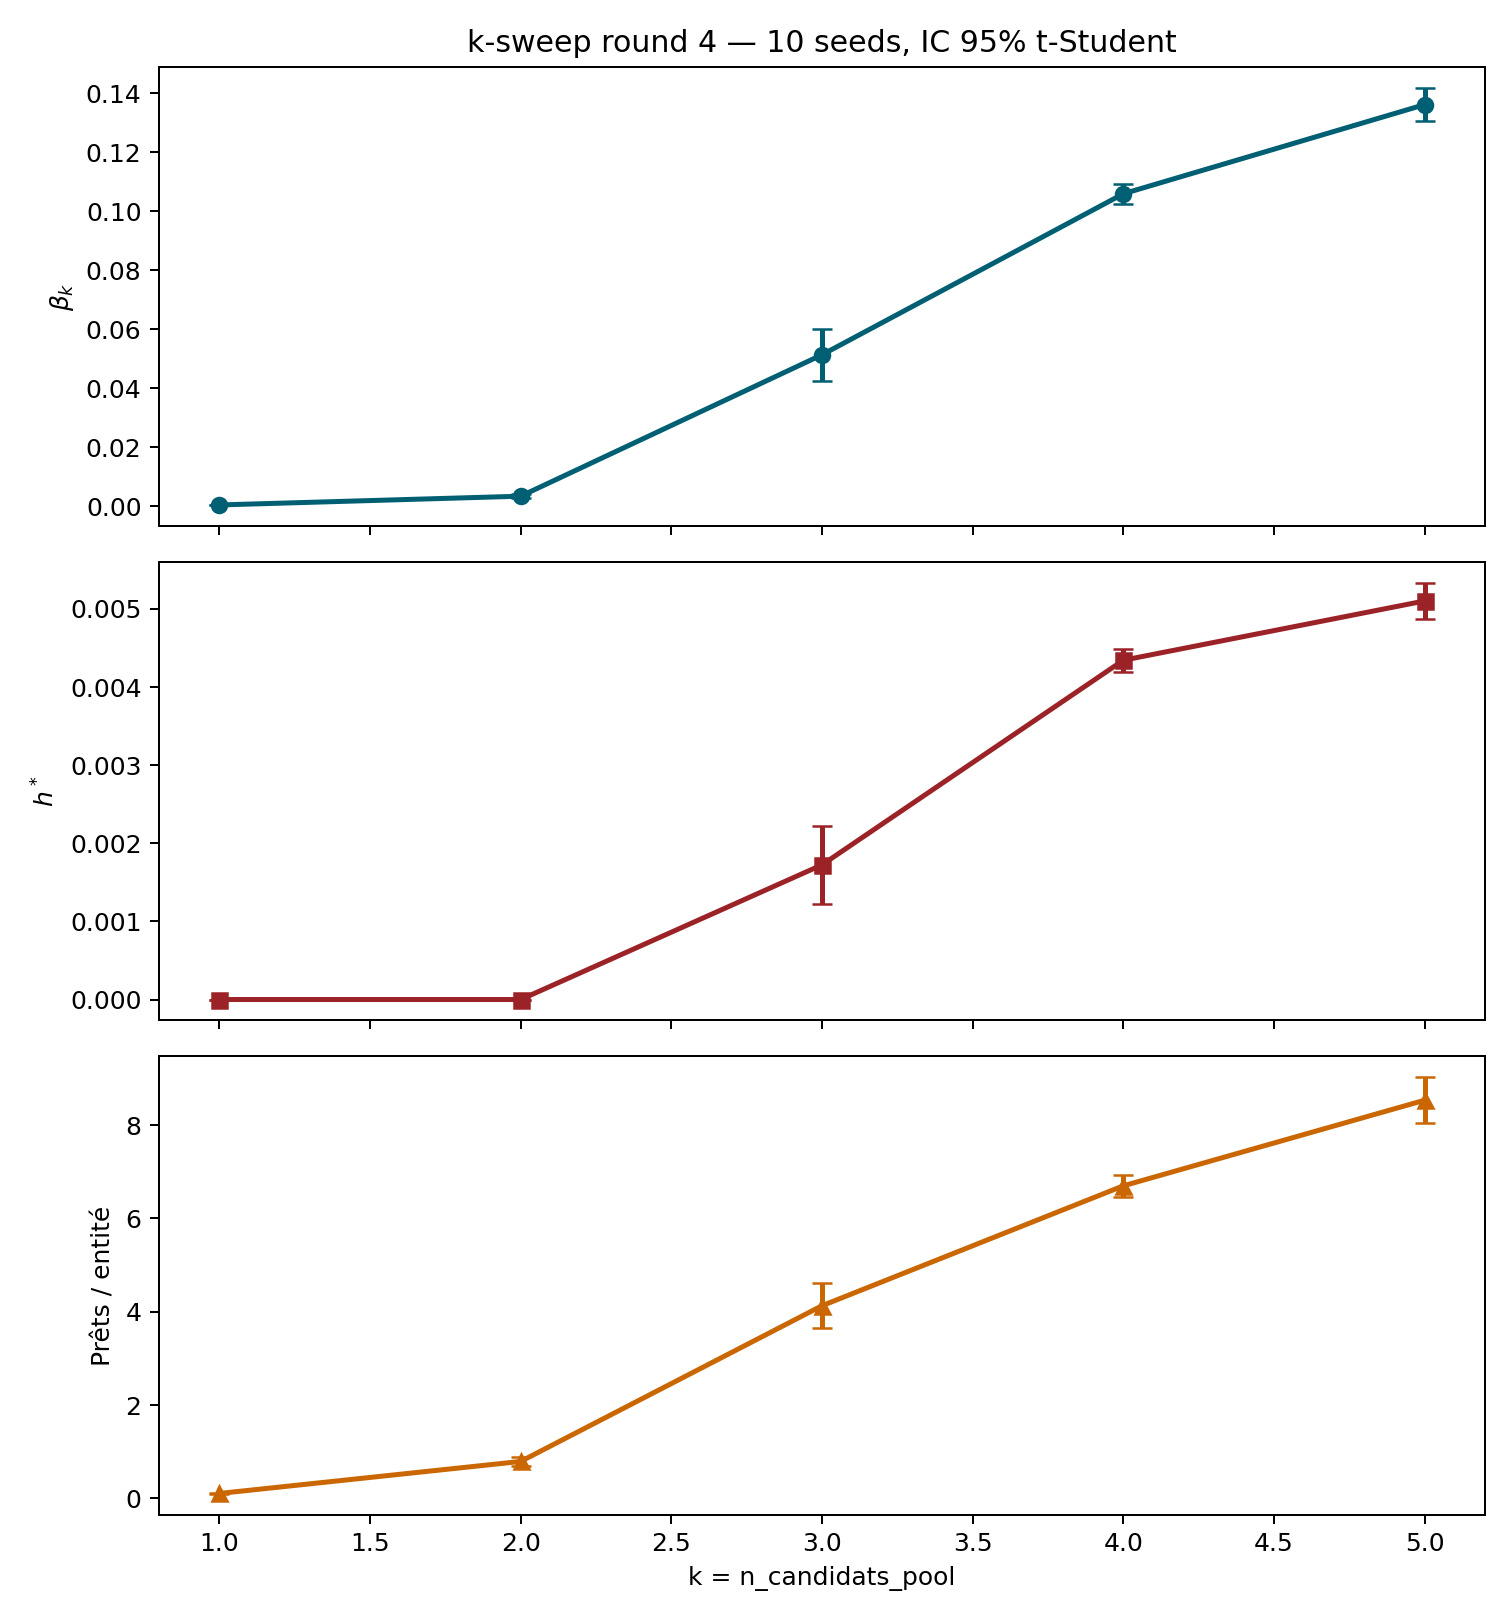
\includegraphics[width=0.92\textwidth]{../data/round4/figures/k_sweep_multiseed_summary.png}
\caption{Sweep round 4 en $k$ sur $10$ seeds. Le saut principal se produit entre $k=2$ et $k=3$: $\beta_k$, le hazard de faillite et la densite de credit changent tous d'ordre de grandeur.}
\label{fig:k-round4}
\end{figure}

\section{Deuxieme pont: point fixe local de population}
Si l'on ne ferme que la dynamique de population,
\[
N_{t+1}-N_t=\Xi_t-F_t,
\]
avec
\[
\mathbb E[\Xi_t]\approx \lambda,
\qquad
\mathbb E[F_t]\approx h^*N_t,
\]
alors un point fixe local naturel est
\[
N^*\approx \frac{\lambda}{h^*}.
\]

Cette fermeture n'a pas de sens quand $h^*$ est pratiquement nul sur l'horizon observe; dans ces cas, la prediction diverge simplement parce que le systeme n'a pas encore developpe un regime de faillite actif. En revanche, sur le sous-ensemble informatif des jeux round 3 avec
\[
h^* \ge 0.002,
\]
on obtient:
\begin{itemize}
\item $19$ runs informatifs;
\item erreur absolue moyenne sur $N_{\mathrm{final}}$: $\approx 55.7$ entites;
\item erreur relative moyenne: $\approx 11.5\%$.
\end{itemize}

Sur la reference longue $(k,\theta,\lambda)=(3,0.35,2)$, seed $42$:
\[
h^*\approx 0.003809,
\qquad
N^*_{\mathrm{pred}}\approx 525.0,
\qquad
N_{\mathrm{final}}=530.
\]
La fermeture est donc tres bonne dans ce regime tardif.

\begin{figure}[t]
\centering
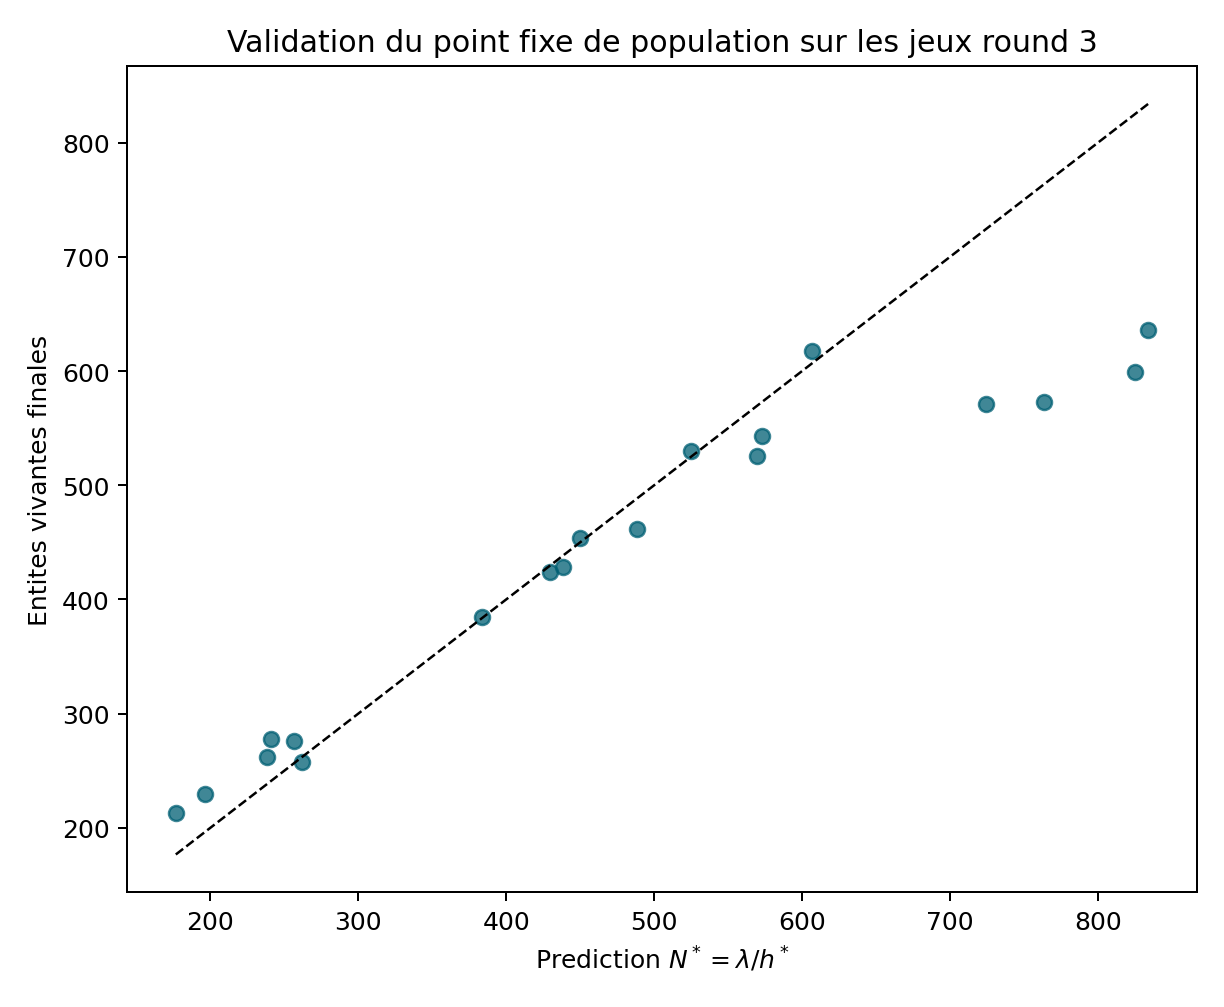
\includegraphics[width=0.78\textwidth]{../data/round4/figures/population_fixed_point_validation.png}
\caption{Validation du point fixe $N^*=\lambda/h^*$ sur les regimes round 3 avec hazard tardif non negligeable. La diagonale trace la prediction parfaite.}
\label{fig:nstar}
\end{figure}

\subsection{Pourquoi le sweep 400 pas et la run 1000 pas divergeaient}
Le round 3 avait une tension apparente entre le sweep a $400$ pas et la reference longue a $1000$ pas. Le round 4 montre que le probleme etait principalement l'horizon, pas les seeds.

Sur les memes seeds $42$--$45$, meme config $(3,0.35,2)$:
\begin{center}
\small
\begin{tabular}{lrrr}
\toprule
Horizon & prets/entite & $\beta$ & $h^*$ \\
\midrule
$400$ pas & $4.178$ & $0.0515$ & $0.00166$ \\
$1000$ pas & $6.934$ & $0.0734$ & $0.00353$ \\
\bottomrule
\end{tabular}
\end{center}

La lecture correcte est donc:
\begin{quote}
a $k=3$, l'horizon $400$ pas reste pre-asymptotique; le quasi-regime dense du WIP apparait beaucoup plus clairement vers l'horizon $1000$.
\end{quote}

\section{Troisieme pont: fermeture correcte de la fragilite cachee}
La quantite exacte est
\[
H=\sum_{e\in\mathcal L} q_e\Big(1-(1-\delta_{\mathrm{exo}})^{a_e}\Big),
\]
et le ratio observe dans les donnees est
\[
\frac{H}{Q},
\qquad
Q=\sum_{e\in\mathcal L} q_e.
\]

La correction decisive du round 4 est conceptuelle:
\begin{itemize}
\item $\delta_{\mathrm{exo}}$ deprecie la \emph{valeur economique} des prets;
\item mais avec $\tau=0$, elle ne supprime pas les prets actifs.
\end{itemize}

Autrement dit, $\delta_{\mathrm{exo}}$ n'est pas le hazard de sortie du portefeuille. Le bon hazard tardif de portefeuille est
\[
\gamma_{\mathrm{loan}}\approx \frac{\beta}{m},
\]
car en quasi-regime de stock,
\[
M_{t+1}-M_t \approx 0
\quad\Rightarrow\quad
\beta N \approx \gamma_{\mathrm{loan}} M
\quad\Rightarrow\quad
\gamma_{\mathrm{loan}}\approx \beta/m.
\]

Si l'age des prets actifs suit alors une loi geometrique
\[
\mathbb P(A=a)\approx \gamma_{\mathrm{loan}}(1-\gamma_{\mathrm{loan}})^a,
\]
on obtient
\[
\frac{H}{Q}
=
1-\mathbb E[(1-\delta_{\mathrm{exo}})^A]
=
1-\frac{\gamma_{\mathrm{loan}}}{1-(1-\gamma_{\mathrm{loan}})(1-\delta_{\mathrm{exo}})}.
\]

Cette fermeture marche remarquablement bien:
\begin{itemize}
\item sur la reference longue seed $42$:
  \[
  \frac{H}{Q}_{\mathrm{obs}} \approx 0.9057,
  \qquad
  \frac{H}{Q}_{\mathrm{pred}} \approx 0.9006;
  \]
\item sur l'ensemble des $46$ runs round 3:
  erreur absolue moyenne $\approx 0.0113$.
\end{itemize}

\begin{figure}[t]
\centering
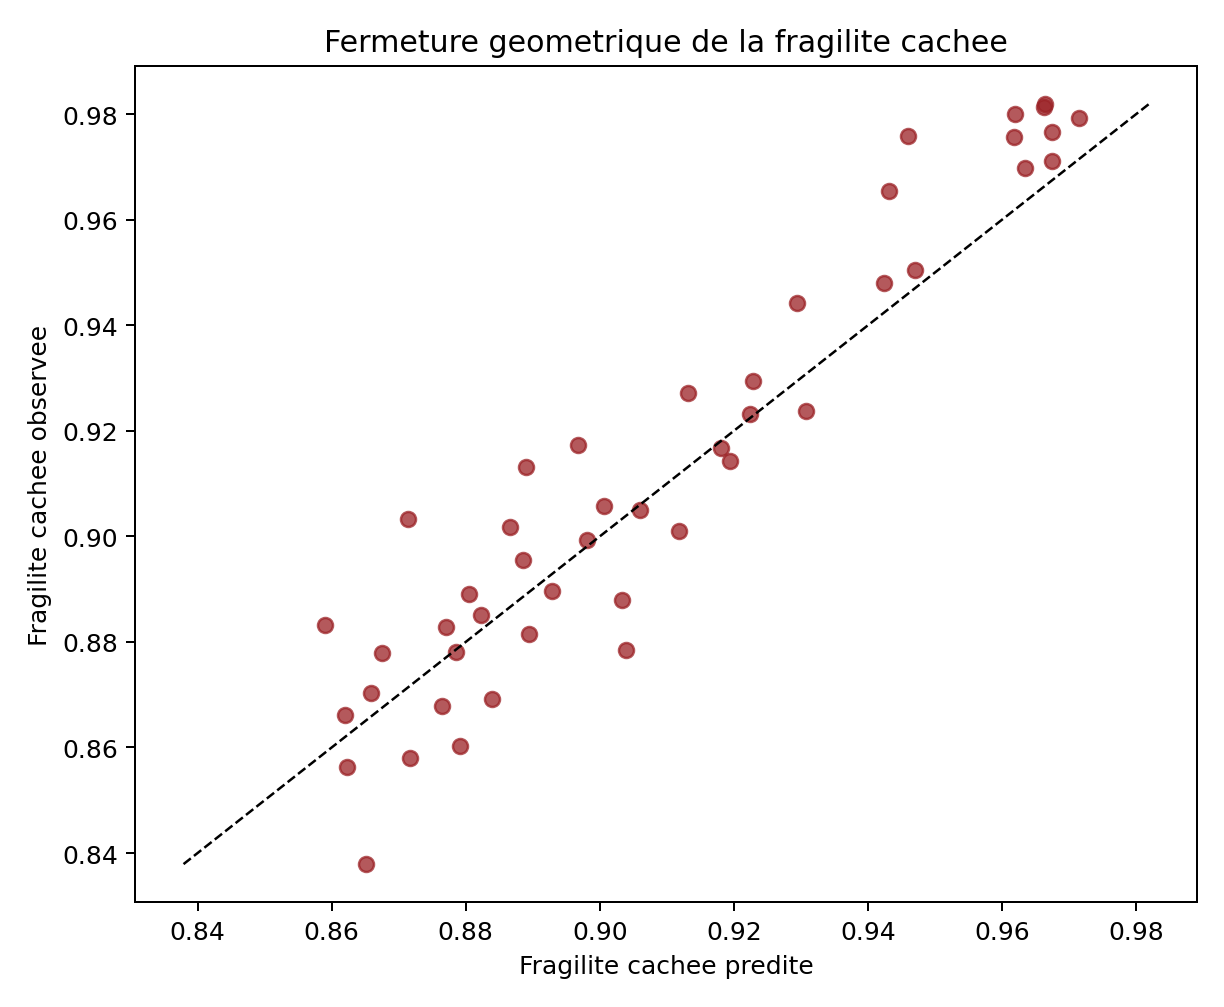
\includegraphics[width=0.78\textwidth]{../data/round4/figures/hidden_fragility_validation.png}
\caption{Validation de la fermeture geometrique correcte de la fragilite cachee. La diagonale trace l'egalite prediction/observation.}
\label{fig:hidden}
\end{figure}

\section{Quatrieme pont: diagnostic spectral effectif}
Le round 4 estime une matrice lineaire d'exposition orientee de l'emprunteur vers le preteur:
\[
(B_t)_{i\leftarrow j}
=
\min\!\left(1,\frac{E_{i\leftarrow j}(t)}{NW_i(t)_+}\right),
\]
ou $E_{i\leftarrow j}(t)$ est l'exposition du preteur $i$ au defaut de l'emprunteur $j$, et $NW_i(t)_+$ la richesse nette positive du preteur au moment du snapshot.

Cette orientation suit la logique du code: un emprunteur qui tombe detruit les actifs du preteur, lequel peut ensuite tomber a son tour s'il est lui-meme emprunteur plus haut dans la chaine.

Sur la run de reference seed $42$:
\begin{center}
\small
\begin{tabular}{lrrr}
\toprule
Fenetre & $\rho(B_t)$ moyen & SCC max moyen & second./fragiles \\
\midrule
$0$--$500$ & $0.107$ & $1.28$ & $0.037$ \\
$500$--$1000$ & $0.422$ & $14.96$ & $0.377$ \\
\bottomrule
\end{tabular}
\end{center}

La structure des cycles change donc vraiment entre la phase precoce et la phase tardive. Le critere spectral n'est plus vide, mais il doit etre lu prudemment:
\begin{itemize}
\item avant $t\approx 500$, le graphe actif reste presque acyclique;
\item apres $t\approx 500$, les boucles apparaissent et $\rho(B_t)$ devient informatif;
\item la propagation empirique reste mieux lue directement par les cascades secondaires que par le seul rayon spectral.
\end{itemize}

\begin{figure}[t]
\centering
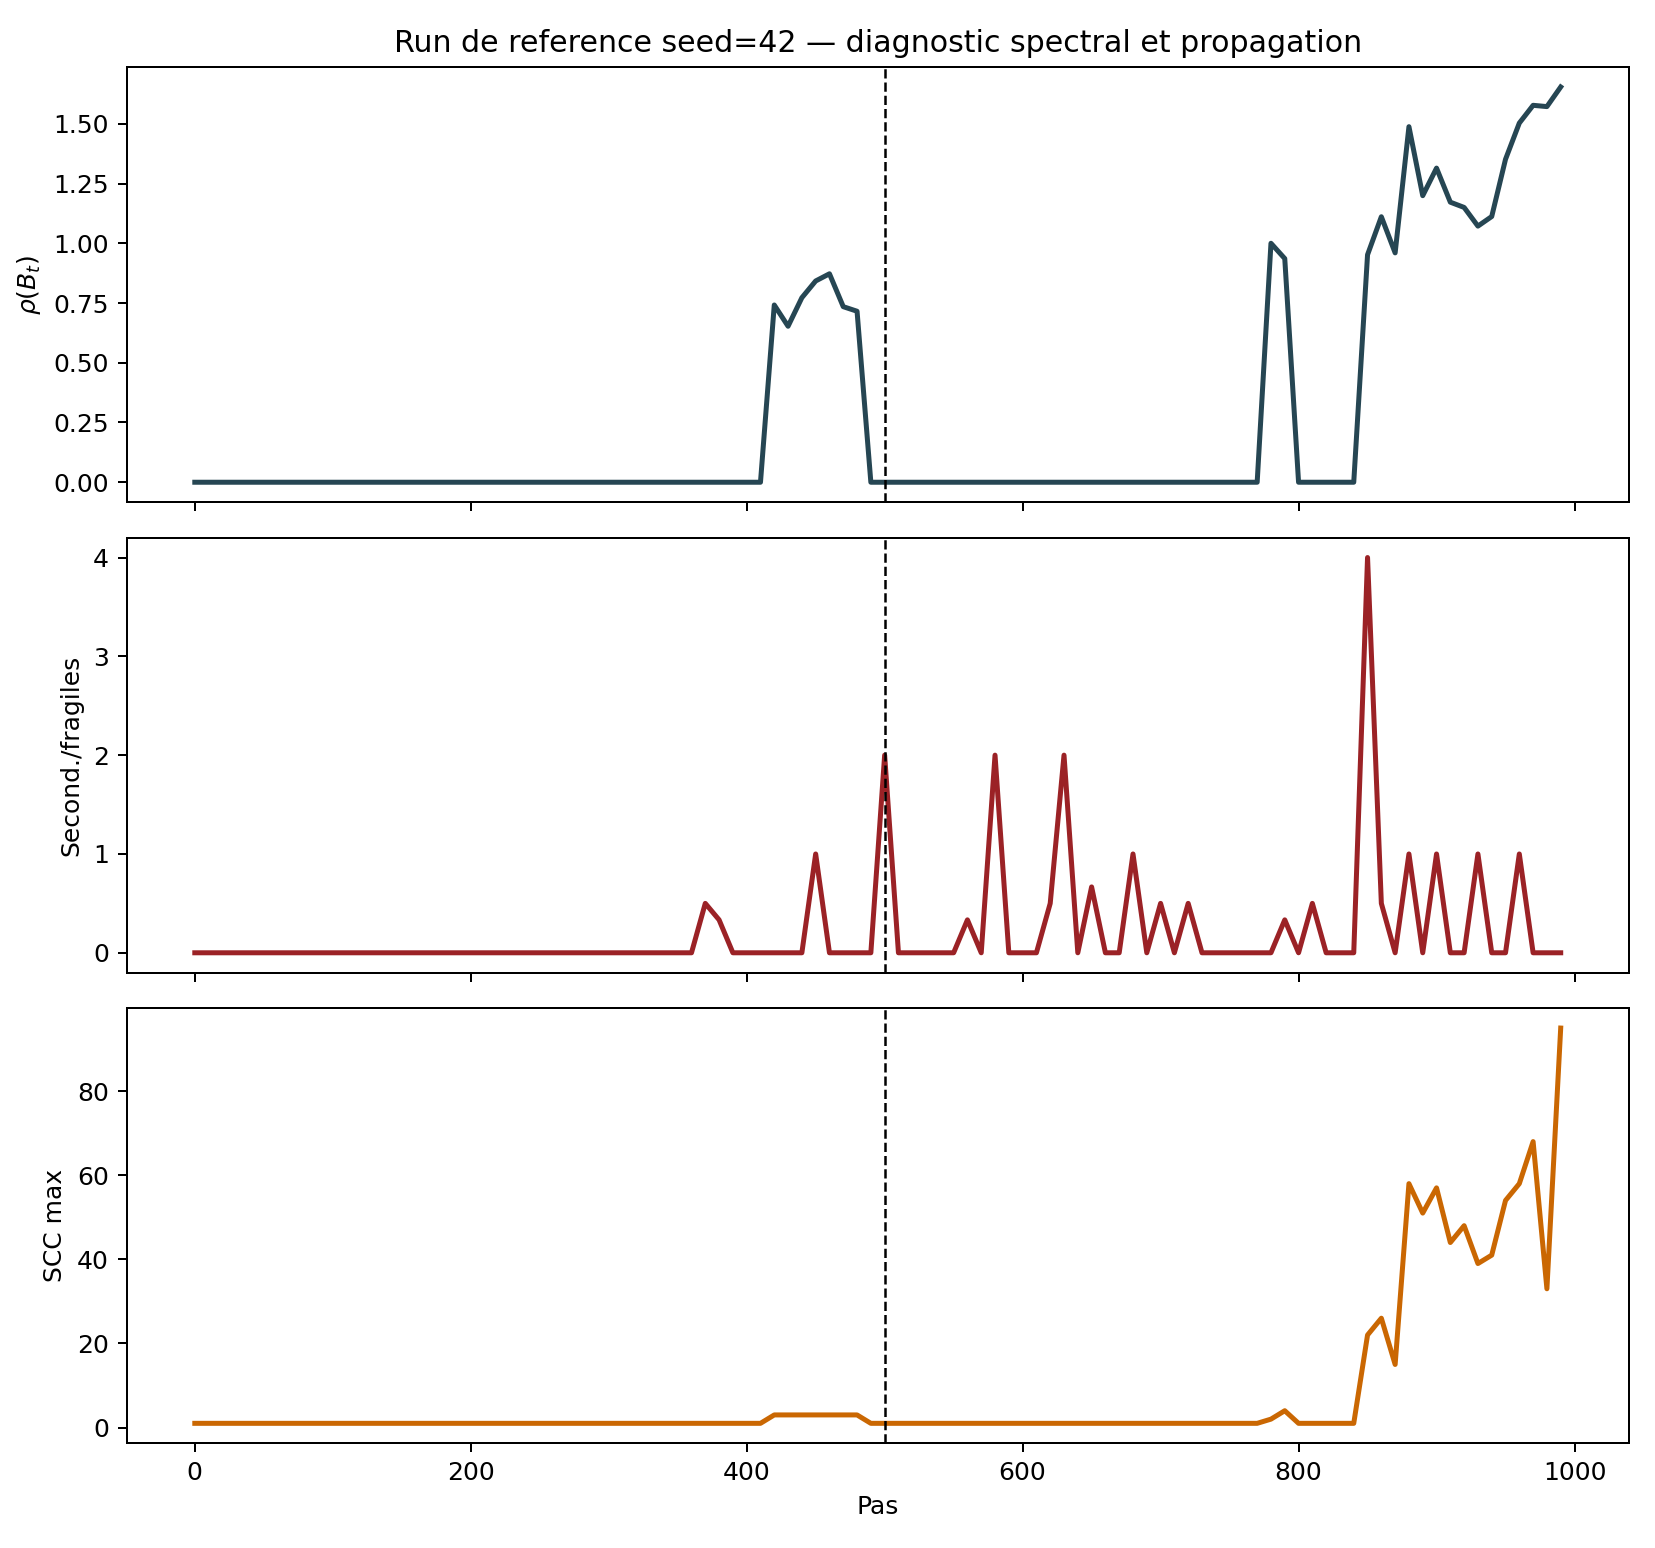
\includegraphics[width=0.92\textwidth]{../data/round4/figures/reference_spectral_timeseries.png}
\caption{Reference round 4. Le diagnostic spectral, la taille de la plus grande composante fortement connexe et la propagation secondaire montent ensemble entre la phase precoce et la fenetre tardive.}
\label{fig:spectral}
\end{figure}

\section{Ce que le round 4 a vraiment ferme}
Le round 4 ne donne pas une formule closee de
\[
(k,\theta,\lambda)\mapsto (m^*, f^*, R_{\mathrm{sec}}^*).
\]
En revanche, il ferme quatre briques qui etaient encore ouvertes:
\begin{itemize}
\item $\beta_k$ comme intensite tardive de formation du credit, avec base multiseed;
\item $N^*=\lambda/h^*$ comme fermeture locale de population;
\item $H/Q$ comme fermeture geometrique correcte du portefeuille de prets;
\item $\rho(B_t)$ comme diagnostic numerique non rhetorique de cyclicite d'exposition.
\end{itemize}

Les deux chantiers majeurs qui restent sont:
\begin{itemize}
\item une vraie fermeture semi-empirique de $\beta_k(k,\theta,\lambda)$ a partir des statistiques d'ordre du marche du credit;
\item une prediction de $m^*$ qui n'utilise pas seulement $\beta$ et $h^*$, mais aussi un modele structurel de survie des prets et de profondeur des chaines de dette.
\end{itemize}

\section{Conclusion}
Le round 4 change la nature du projet plus qu'il n'en change le vocabulaire. On ne dit plus seulement ``la carte empirique suggere tel regime''. On peut maintenant dire:
\begin{itemize}
\item le seuil principal du marche de credit est bien entre $k=2$ et $k=3$, et il se voit directement sur $\beta_k$;
\item la population tardive est deja approximativement reglee par $N^*=\lambda/h^*$ dans les regimes ou les cascades sont actives;
\item la fragilite cachee tardive est expliquee quantitativement par le hazard de sortie des prets, non par la seule depreciation comptable;
\item la structure cyclique du graphe de credit n'est pas une metaphore: elle devient mesurable et augmente effectivement en regime tardif.
\end{itemize}

Ce n'est pas encore une theorie fermee du WIP. C'est en revanche le premier round ou certaines predictions peuvent etre ecrites, chiffrees, puis confrontees directement aux donnees du modele.

\end{document}
